% Source: TeX Live 2025, doc/generic/pgf/pgfmanual-en-tikz-plots.tex:710-716
% (the two inline ybar series). Keep the five sample positions, magnitudes
% and manual's 6pt / 4pt widths and 3pt shift; signs and solid fills are
% adapted to show gains and losses on opposite sides of a visible zero line.
\documentclass[border=2pt]{standalone}
\usepackage{tikz}
\begin{document}
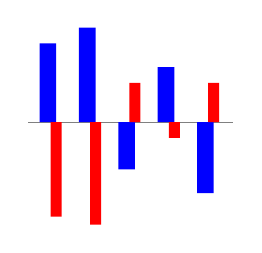
\begin{tikzpicture}
  \draw[gray] (-0.25,0) -- (2.35,0);
  \fill[blue,bar width=6pt] plot[ybar]
    coordinates {(0,1) (0.5,1.2) (1,-0.6) (1.5,0.7) (2,-0.9)};
  \fill[red,bar width=4pt,bar shift=3pt] plot[ybar]
    coordinates {(0,-1.2) (0.5,-1.3) (1,0.5) (1.5,-0.2) (2,0.5)};
\end{tikzpicture}
\end{document}
